% CSUF MPA Orientation
% Author: David Adams

\documentclass[10pt]{beamer}
\usetheme[numbering=fraction,progressbar=frametitle]{metropolis}
% Handout mode toggle
\newif\ifhandout
\ifhandout
  \documentclass[handout]{beamer}
  \usepackage{pgfpages}
  \pgfpagesuselayout{4 on 1}[letterpaper, landscape]
\fi

% --------------------
% Packages
% --------------------
\usepackage{booktabs}
\usepackage{tabularx}
\usepackage{calc}
\usepackage{tikz}
\usepackage{ifluatex}
\usepackage{microtype}
\usepackage[utf8]{inputenc}
\usepackage{csquotes}
\usepackage{qrcode}
\usepackage{hyperref}
\hypersetup{
  colorlinks=true,
  linkcolor=black,
  urlcolor=black
}
\urlstyle{same}
\usepackage{etoolbox} % for \ifdefempty (already in TL)
% print #1 followed by a paragraph break only if not empty
\newcommand{\ShowIfNonempty}[1]{\ifdefempty{#1}{}{#1\par}}


% --------------------
% Fonts (LuaLaTeX/XeLaTeX preferred; pdfLaTeX falls back automatically)
% --------------------
\ifluatex
  \usepackage{fontspec}
  \setsansfont[
    Ligatures=TeX,
    Scale=0.96,
  ]{TeX Gyre Heros} % swap to Inter, Source Sans 3, or your campus font if installed
\else
  \usepackage[T1]{fontenc}
  \usepackage[utf8]{inputenc}
  \usepackage{lmodern}
\fi

% --------------------
% CSUF brand colors
% --------------------
\definecolor{titanblue}{HTML}{00244E}
\definecolor{mediumblue}{HTML}{0F3F8C}
\definecolor{skyblue}{HTML}{EBFBFF}
\definecolor{titanorange}{HTML}{FF7900}
\definecolor{titangray}{HTML}{F5F5F5}
\definecolor{titantext}{HTML}{222222}

% --------------------
% Metropolis color + font tweaks (high-contrast, large room friendly)
% --------------------
\setbeamercolor{normal text}{fg=titantext,bg=white}
\setbeamercolor{alerted text}{fg=titanorange}
\setbeamercolor{example text}{fg=mediumblue}

\setbeamercolor{title}{fg=titanblue}
\setbeamercolor{subtitle}{fg=mediumblue}
\setbeamercolor{frametitle}{fg=white,bg=titanblue}
\setbeamercolor{progress bar}{fg=titanorange,bg=titangray}
\setbeamercolor{block title}{fg=white,bg=titanblue}
\setbeamercolor{block body}{fg=titantext,bg=skyblue!12}

\setbeamerfont{title}{size=\Large,series=\bfseries}
\setbeamerfont{frametitle}{size=\large,series=\bfseries}
\setbeamerfont{block title}{series=\bfseries}

% Section break slides
\setbeamercolor{background canvas}{bg=white} % keep canvas white everywhere
\setbeamercolor{standout}{bg=titanblue, fg=titanorange} % section/title slides with orange text
\setbeamercolor{palette primary}{bg=titanblue, fg=titanorange} % for section pages
\setbeamercolor{section title}{fg=titanorange} % explicitly set section title color
\setbeamercolor{section page}{bg=titanblue, fg=titanorange} % section page colors

% Additional metropolis-specific color overrides
\setbeamercolor{section in toc}{fg=titanorange}
\setbeamercolor{subsection in toc}{fg=titanorange}
\setbeamercolor{title in head/foot}{fg=titanorange}
\setbeamercolor{author in head/foot}{fg=titanorange}
\setbeamercolor{date in head/foot}{fg=titanorange}

% Override metropolis section page template colors
\AtBeginDocument{
  \setbeamercolor{section title}{fg=titanorange}
  \setbeamercolor{palette primary}{fg=titanorange, bg=titanblue}
}

% (Optional) tweak section page style if you like:
\metroset{sectionpage=progressbar} % or sectionpage=none/simple
% Add progress bar
\makeatletter
\setbeamertemplate{headline}{%
  \begin{beamercolorbox}[wd=\paperwidth,ht=0.4cm,dp=0cm]{titanblue}%
    \begin{tikzpicture}
      \fill[titanorange] (0,0) rectangle (\the\paperwidth*\insertframenumber/\inserttotalframenumber,0.4cm);
    \end{tikzpicture}%
  \end{beamercolorbox}%
}
\makeatother

% --------------------
% Title metadata
% --------------------
\title{Master of Public Administration Program}
\subtitle{MPA Student Orientation}
\date{Fall 2025}
\titlegraphic{\vspace{-0.75em}
\includegraphics[width=.75\textwidth]{images/PUBLIC-ADMINISTRATION-color2.png}}

% --------------------
% Helpful utilities
% --------------------
% Section title slides
% Force all section slides to use orange text on blue background and \huge size
\AtBeginSection[]{
  {\setbeamercolor{background canvas}{bg=titanblue}%
   \setbeamercolor{standout}{bg=titanblue, fg=titanorange}%
   \setbeamercolor{section title}{fg=titanorange}%
   \begin{frame}[standout]
     \centering
     {\huge\textcolor{titanorange}{\insertsection}}
   \end{frame}}
}

% Uniform image height for faculty cards
\newlength{\imageheight}
\setlength{\imageheight}{3.4cm}

% Compact two-column list frame
\newenvironment{twocolbullets}
{\begin{columns}[T,onlytextwidth]\column{0.5\textwidth}\begin{itemize}}
{\end{itemize}\column{0.5\textwidth}\begin{itemize}\end{itemize}\end{columns}}

% A small "key dates" helper
\newcommand{\KeyDate}[2]{\textbf{#1:} #2\par}

% --------------------
\begin{document}
% --------------------

\maketitle

\section{\textcolor{titanorange}{Welcome}}
\begin{frame}{Agenda}
\begin{columns}[T,totalwidth=\textwidth]
  \begin{column}{0.33\textwidth}
    \textbf{Large Group}
    \begin{itemize}\setlength{\itemsep}{2pt}
      \item Welcome and Introductions
      \item Why CSUF?
      \item Mission, Vision, Values
      \item Public Administration Student Association (PASA)
    \end{itemize}
  \end{column}

  \begin{column}{0.33\textwidth}
    \textbf{Breakouts}
    \begin{enumerate}\setlength{\itemsep}{2pt}
      \item \textbf{New Students}
        \begin{itemize}\setlength{\itemsep}{1pt}
          \item Faculty Profiles
          \item Curriculum
          \item Milestones
          \item Scholarships and Awards
        \end{itemize}
      \item \textbf{Family, Alums, Current Students}
        \begin{itemize}\setlength{\itemsep}{1pt}
          \item Supporting your MPA Student
          \item Navigating Grad School
          \item Success Strategies
        \end{itemize}
    \end{enumerate}
  \end{column}

  \begin{column}{0.33\textwidth}
    \textbf{Large Group}
    \begin{itemize}\setlength{\itemsep}{2pt}
      \item Success and Support
      \item Campus Resources
      \item Contact Information
      \item Large Group Q\&A
    \end{itemize}
  \end{column}
\end{columns}
\end{frame}

\section{\textcolor{titanorange}{Introductions}}

\section{\textcolor{titanorange}{Why CSUF}}
\begin{frame}{Program by the Numbers}
\begin{Large}
\begin{itemize}
  \item \textbf{1968:} Year the program began awarding degrees
  \item \textbf{1:} The only public MPA program in Orange County
  \item \textbf{93:} Current students enrolled Fall 2025
  \item \textbf{\(\sim\)30:} Graduates each year
  \item \textbf{4:} Concentrations offered
  \item \textbf{3 years:} Typical time to degree
\end{itemize}
\end{Large}
\end{frame}

\begin{frame}{The Value of a CSUF MPA}
\begin{Large}
\begin{itemize}
  \item \#1: \textbf{Most selective public MPA program} in Southern California
  \item \textbf{6.4:1} student--faculty ratio (lowest among SoCal public MPAs)
  \item \textbf{1,200+ alumni} leading in government, nonprofit, and private sectors
  \item \textbf{NASPAA accredited} continuously since the 1980s
    \begin{itemize}
      \item Reaccredited for 6 years (2025)
      \item Recognized for excellence and commitment to public service
    \end{itemize}
\end{itemize}
\end{Large}
\end{frame}

\section{\textcolor{titanorange}{Mission, Vision, Values}}

\begin{frame}{Our Mission and Vision}
\textbf{Mission}\\
We prepare leaders to address complex social issues, uphold democratic values, and foster ethical, equitable, and inclusive public service in Orange County and beyond.

\vspace{0.8em}
\textbf{Vision}\\
To be recognized for excellence in value-driven public service and community engagement.
\end{frame}

\begin{frame}{Our Values}
\textbf{Values}
\begin{description}
  \item[Accountability] Promoting democratic transparency, responsiveness, and evidence-informed decision-making to uphold public trust and integrity.
  \item[Ethics] Advancing integrity, fairness, and service to the public good by fostering ethical reasoning and critical awareness in public administration.
  \item[Collaboration] Cultivating collaborative skills for cross-sector partnerships, networked governance, and inclusive stakeholder engagement.
  \item[Lifelong Learning] Instilling habits of continuous learning, reflective practice, and professional development to support adaptive leaders and long-term impact.
\end{description}
\end{frame}

\section{\textcolor{titanorange}{Public Administration Student Association (PASA)}}

\begin{frame}{Public Administration Student Association (PASA)}
  \centering
  
\includegraphics[width=\textwidth]{images/join_PASA.png}
\end{frame}

\section{\textcolor{titanorange}{Breakout Groups}}

\begin{frame}{Breakout Groups}
\begin{columns}[T,onlytextwidth]
  \column{0.45\textwidth}
  \textbf{Breakout Group 1: New Students}
  \begin{itemize}
    \item Program structure
    \item Concentrations
    \item Milestones
  \end{itemize}

  \column{0.55\textwidth}
  \textbf{Breakout Group 2: Family, Alums, Current Students}
  \begin{itemize}
    \item Supporting your MPA Student
    \item Understanding the program
    \item Navigating Grad School
    \item Success Strategies
  \end{itemize}
\end{columns}
\end{frame}

\section{\textcolor{titanorange}{Faculty}}
\begin{frame}{MPA Program Faculty}
\begin{columns}[T,onlytextwidth]
  \column{0.64\textwidth}
  \textbf{Core Faculty}
  \begin{itemize}
    \item Eight full-time faculty members
    \item Diverse research and strong professional experience
    \item Active in scholarship and community engagement
  \end{itemize}
  \column{0.36\textwidth}
  \includegraphics[height=\imageheight]{images/gordon_hall.jpg}
\end{columns}
\end{frame}

% Faculty profiles using individual frames instead of problematic macro
\begin{frame}{David P. Adams, Ph.D.}
\begin{columns}[T,onlytextwidth]
  \column{0.66\textwidth}
    \raggedright
    {\large\bfseries David P. Adams, Ph.D.}\par
    {Associate Professor \& MPA Director}\par
    {\footnotesize At CSUF since 2016 \quad | \quad Ph.D., Auburn University}\par\vspace{0.4em}

    \textbf{Research}
    \begin{itemize}
      \item Public policy outcomes
      \item Collaboration
      \item Environmental \& energy policy
      \item Environmental justice
    \end{itemize}

    \textbf{Courses}
    \begin{itemize}
      \item Foundations of PA
      \item Capstone Seminar
      \item Collaborative Governance
    \end{itemize}

  \column{0.34\textwidth}
    \vspace*{0.25cm}
    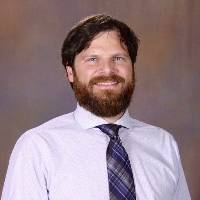
\includegraphics[height=\imageheight]{images/adams.jpg}
\end{columns}
\end{frame}

\begin{frame}{Shelly Arsneault, Ph.D.}
\begin{columns}[T,onlytextwidth]
  \column{0.66\textwidth}
    \raggedright
    {\large\bfseries Shelly Arsneault, Ph.D.}\par
    {Professor; Vice Chair of PAJ}\par
    {\footnotesize At CSUF since 2002 \quad | \quad Ph.D., Michigan State University}\par\vspace{0.4em}

    \textbf{Research}
    \begin{itemize}
      \item Nonprofit management
      \item Education policy
    \end{itemize}

    \textbf{Courses}
    \begin{itemize}
      \item Foundations of PA
      \item Nonprofit Management
      \item Education Policy
    \end{itemize}

  \column{0.34\textwidth}
    \vspace*{0.25cm}
    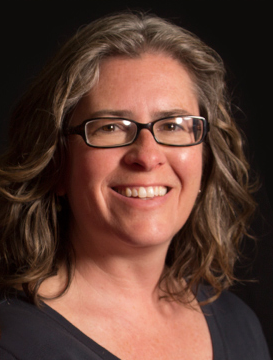
\includegraphics[height=\imageheight]{images/arsneault.png}
\end{columns}
\end{frame}

\begin{frame}{Sean Angst, Ph.D.}
\begin{columns}[T,onlytextwidth]
  \column{0.66\textwidth}
    \raggedright
    {\large\bfseries Sean Angst, Ph.D.}\par
    {Assistant Professor}\par
    {\footnotesize At CSUF since 2024 \quad | \quad Ph.D., USC Price}\par\vspace{0.4em}

    \textbf{Research}
    \begin{itemize}
      \item Housing policy
      \item Community development
      \item Racial justice
    \end{itemize}

    \textbf{Courses}
    \begin{itemize}
      \item Administrative Research \& Analysis
      \item Policy Analysis
    \end{itemize}

  \column{0.34\textwidth}
    \vspace*{0.25cm}
    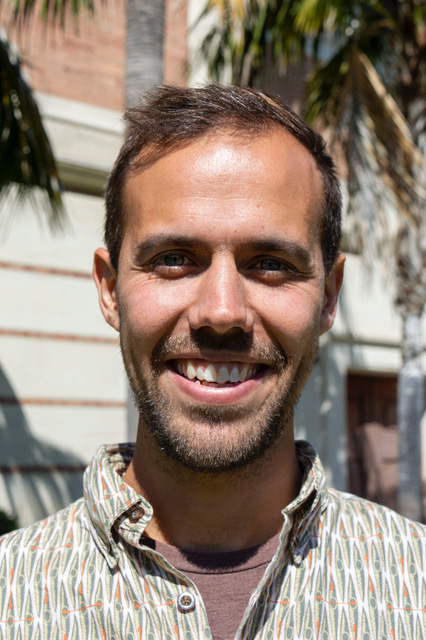
\includegraphics[height=\imageheight]{images/angst.jpg}
\end{columns}
\end{frame}

\begin{frame}{Meriem Doucette, Ph.D.}
\begin{columns}[T,onlytextwidth]
  \column{0.66\textwidth}
    \raggedright
    {\large\bfseries Meriem Doucette, Ph.D.}\par
    {Associate Professor}\par
    {\footnotesize At CSUF since 2015 \quad | \quad Ph.D., University of Georgia}\par\vspace{0.4em}

    \textbf{Research}
    \begin{itemize}
      \item Organizational theory
      \item Change management
    \end{itemize}

    \textbf{Courses}
    \begin{itemize}
      \item Organizational Theory
      \item Ethics
      \item Organizational Development
      \item Leadership
    \end{itemize}

  \column{0.34\textwidth}
    \vspace*{0.25cm}
    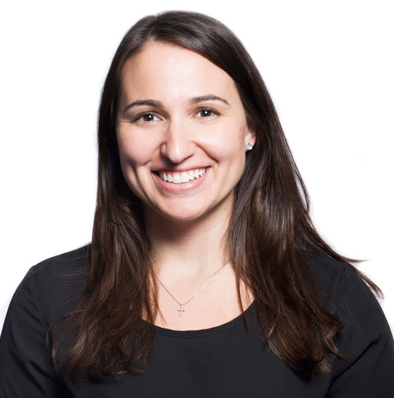
\includegraphics[height=\imageheight]{images/doucette.png}
\end{columns}
\end{frame}

\begin{frame}{Elaine Frey, Ph.D.}
\begin{columns}[T,onlytextwidth]
  \column{0.66\textwidth}
    \raggedright
    {\large\bfseries Elaine Frey, Ph.D.}\par
    {Professor}\par
    {\footnotesize Ph.D., George Washington University}\par\vspace{0.4em}

    \textbf{Research}
    \begin{itemize}
      \item Environmental economics
      \item Energy economics
      \item Applied microeconomics
    \end{itemize}

    \textbf{Courses}
    \begin{itemize}
      \item Environmental Policy
      \item Administrative Research \& Analysis
    \end{itemize}

  \column{0.34\textwidth}
    \vspace*{0.25cm}
    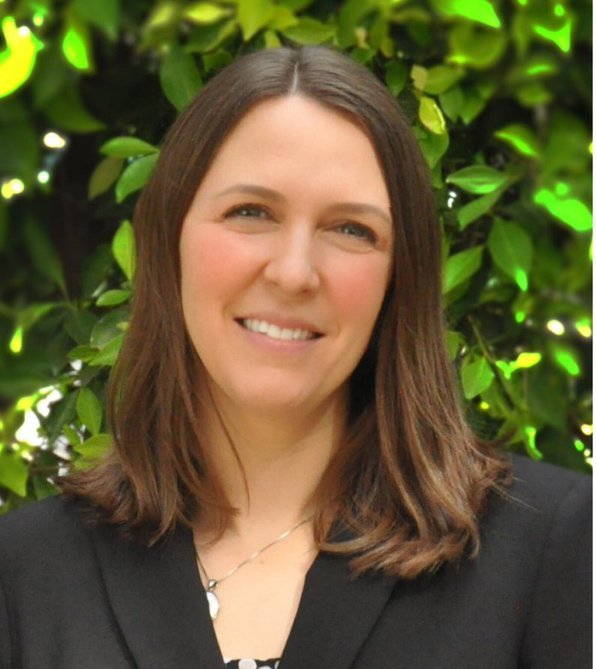
\includegraphics[height=\imageheight]{images/frey.jpg}
\end{columns}
\end{frame}

\begin{frame}{Sarah A. Hill, Ph.D.}
\begin{columns}[T,onlytextwidth]
  \column{0.66\textwidth}
    \raggedright
    {\large\bfseries Sarah A. Hill, Ph.D.}\par
    {Professor}\par
    {\footnotesize At CSUF since 2007 \quad | \quad Ph.D., Caltech}\par\vspace{0.4em}

    \textbf{Research}
    \begin{itemize}
      \item Elections administration
      \item Education policy
    \end{itemize}

    \textbf{Courses}
    \begin{itemize}
      \item State \& Local Government
      \item Public Policy
      \item Diversity in Public Management
    \end{itemize}

  \column{0.34\textwidth}
    \vspace*{0.25cm}
    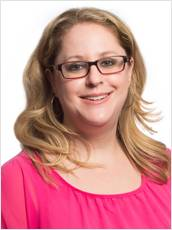
\includegraphics[height=\imageheight]{images/hill.jpg}
\end{columns}
\end{frame}

\begin{frame}{Myung--Jung ``MJ'' Kwon, Ph.D.}
\begin{columns}[T,onlytextwidth]
  \column{0.66\textwidth}
    \raggedright
  {\large\bfseries Myung--Jung ``MJ'' Kwon, Ph.D.}\par
    {Professor; MPA Advisor}\par
    {\footnotesize At CSUF since 2009 \quad | \quad Ph.D., Florida State University}\par\vspace{0.4em}

    \textbf{Research}
    \begin{itemize}
      \item Public sector innovation
      \item E-government
    \end{itemize}

    \textbf{Courses}
    \begin{itemize}
      \item Human Resources Management
      \item Public Personnel Administration
      \item Diversity in Public Management
    \end{itemize}

  \column{0.34\textwidth}
    \vspace*{0.25cm}
    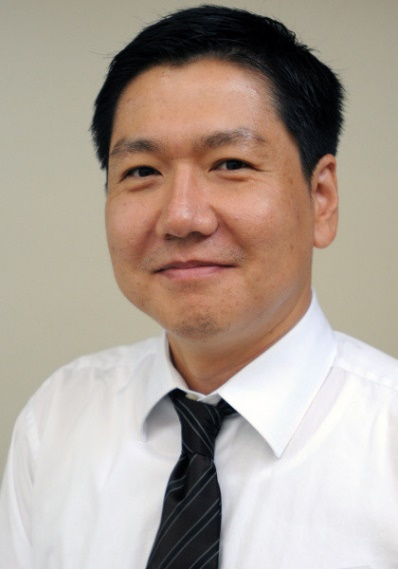
\includegraphics[height=\imageheight]{images/kwon.jpg}
\end{columns}
\end{frame}

\begin{frame}{Samuel B. Stone, Ph.D.}
\begin{columns}[T,onlytextwidth]
  \column{0.66\textwidth}
    \raggedright
    {\large\bfseries Samuel B. Stone, Ph.D.}\par
    {Professor}\par
    {\footnotesize At CSUF since 2011 \quad | \quad Ph.D., Indiana University}\par\vspace{0.4em}

    \textbf{Research}
    \begin{itemize}
      \item Financial analysis
      \item Fiscal policy
      \item Local government management
    \end{itemize}

    \textbf{Courses}
    \begin{itemize}
      \item Public Finance
      \item Public Budgeting
      \item Local Government Management
    \end{itemize}

  \column{0.34\textwidth}
    \vspace*{0.25cm}
    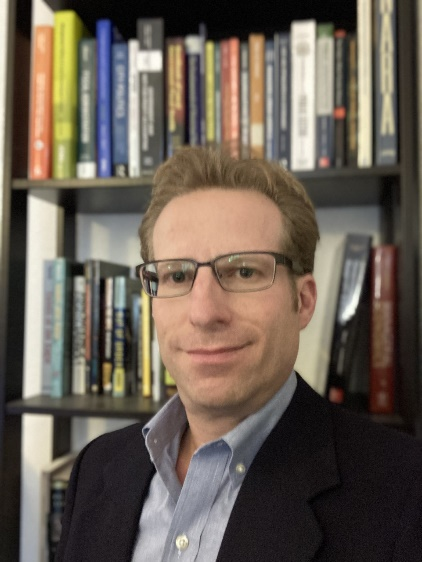
\includegraphics[height=\imageheight]{images/stone.jpg}
\end{columns}
\end{frame}

\begin{frame}{Scott Spitzer, Ph.D.}
\begin{columns}[T,onlytextwidth]
  \column{0.66\textwidth}
    \raggedright
    {\large\bfseries Scott Spitzer, Ph.D.}\par
    {Affiliated Faculty; Professor}\par
    {\footnotesize At CSUF since 2006 \quad | \quad Ph.D., Columbia University}\par\vspace{0.4em}

    \textbf{Research}
    \begin{itemize}
      \item Urban politics
      \item Racial politics
      \item Social welfare
    \end{itemize}

    \textbf{Courses}
    \begin{itemize}
      \item Urban Politics
      \item Metropolitan Politics \& Policy
    \end{itemize}

  \column{0.34\textwidth}
    \vspace*{0.25cm}
    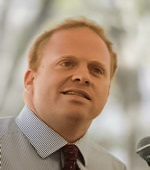
\includegraphics[height=\imageheight]{images/spitzer.png}
\end{columns}
\end{frame}

\section{\textcolor{titanorange}{Curriculum}}

\begin{frame}{Program Structure}
\begin{itemize}
  \item \textbf{Total Units: 36} (12 courses)
  \item Prerequisites
  \item Core courses
  \item One concentration
  \item Electives
  \item Internship (required if no public sector experience)
  \item Comprehensive Exam (embedded in Capstone)
\end{itemize}
\end{frame}

\begin{frame}{Concentrations}
Choose one concentration:
\begin{itemize}
  \item Human Resource Management
  \item Local Government Management
  \item Public Finance
  \item Public Policy
\end{itemize}
\emph{Tip:} Choose a concentration that complements your role and goals.
\end{frame}

\section{\textcolor{titanorange}{Milestones}}
\begin{frame}{Program Milestones Overview}
\centering
\textbf{Your Path to Success}\\[4pt]
\small This timeline represents typical progression. Your path may vary; meet with the MPA advisor to build your sequence.
\end{frame}

\begin{frame}{Program Orientation}
\textbf{Prior to First Semester}
\begin{itemize}
  \item Attend orientation
  \item Review student handbook \small(\url{https://csuf-mpa.github.io/mpa_handbook/})
  \item Complete required paperwork
\end{itemize}
\textbf{Resources}
\begin{itemize}
  \item Academic calendar \small(\url{https://apps.fullerton.edu/AcademicCalendar/})
  \item Campus map \small(\url{https://www.fullerton.edu/campusmap/})
\end{itemize}
\end{frame}

\begin{frame}{First Semester Foundations}
\textbf{Semester One}
\begin{itemize}
  \item Complete POSC 509: Foundations of Public Administration
  \item Take one additional core
\end{itemize}
\begin{itemize}
  \item \alert{Important:} Take POSC 509 in your first (or second) term.
  \item \alert{Tip:} Use this semester to build foundational knowledge and skills.
  \item \alert{Recommendation:} Join PASA, the Public Administration Student Association.
\end{itemize}
\end{frame}

\begin{frame}{Program Planning}
\textbf{Semester Two}
\begin{itemize}
  \item Meet with the MPA advisor
  \item Declare concentration
  \item Complete two core courses
  \item Map your timeline to completion
\end{itemize}
\end{frame}

\begin{frame}{Mid-Program Achievement}
\textbf{At 18 Units}
\begin{itemize}
  \item Maintain 3.0+ GPA
  \item Consider \emph{Pi Alpha Alpha} (3.7+ GPA)
  \item Progress review with advisor
\end{itemize}
\end{frame}

\begin{frame}{Advanced Phases}
\textbf{Years 2--3}
\begin{itemize}
  \item Finish three concentration courses
  \item Complete remaining core
\end{itemize}
\textbf{Capstone Prep (Penultimate Semester)}
\begin{itemize}
  \item Verify prerequisites
  \item Enroll in POSC 521 (Capstone) for final semester
  \item Begin comprehensive exam prep
\end{itemize}
\end{frame}

\begin{frame}{Final Steps}
\textbf{Final Semester}
\begin{itemize}
  \item File graduation check
    \begin{itemize}
      \item Spring deadline: early February
      \item Fall deadline: early September
    \end{itemize}
  \item Complete Capstone and comprehensive exam
  \item Submit required documentation
  \item Register for commencement
\end{itemize}
\end{frame}

\section{\textcolor{titanorange}{Scholarships \& Awards}}
\begin{frame}{Scholarships \& Awards}
\begin{itemize}
  \item Lawson Internship in Public Service Award
    \begin{itemize}
      \item \$2{,}000 for MPA student in 497
      \item Fall \& Spring; Spring deadline: Feb 1
    \end{itemize}
  \item Alan Saltzstein Excellence Award
    \begin{itemize}
      \item \$1{,}000 (6--12 units)
      \item Fall \& Spring
    \end{itemize}
  \item MPA Alumni Scholarship
    \begin{itemize}
      \item \$1{,}000 for first-semester students
      \item Fall only (awarded in Spring)
    \end{itemize}
\end{itemize}
\end{frame}

\begin{frame}{Graduation Awards}
\begin{itemize}
  \item Sidney Baldwin Award (MPA Outstanding Student)
    \begin{itemize}
      \item Based on GPA \& Comprehensive Exam
    \end{itemize}
  \item Outstanding Public Administration Undergraduate
  \item Spirit of Public Service Award
  \item Irving Stone Best Paper Award
\end{itemize}
\end{frame}

\section{\textcolor{titanorange}{Success \& Support}}
\begin{frame}{Keys to Graduate School Success}
\begin{columns}[T,onlytextwidth]
  \column{0.5\textwidth}
  \textbf{Academic}
  \begin{itemize}
    \item Start assignments early
    \item Study groups
    \item Keep detailed cross-course notes
    \item Use office hours
    \item Protect work--life--school balance
  \end{itemize}
  \column{0.5\textwidth}
  \textbf{Professional}
  \begin{itemize}
    \item Network with classmates
    \item Join associations
    \item Consider Pi Alpha Alpha (3.7+)
    \item Build faculty relationships
    \item Start career planning now
  \end{itemize}
\end{columns}

\vspace{0.4em}
\textbf{Time Management}
\begin{itemize}
  \item Plan \(\approx\) 3 hours of study per course hour
  \item Track deadlines
  \item Break big projects into small, dated tasks
\end{itemize}
\end{frame}

\section{\textcolor{titanorange}{Q \& A}}


\section{\textcolor{titanorange}{End of Breakout}}
\begin{frame}[standout]
\centering
\huge{Return to Main Session}
\end{frame}


\section{\textcolor{titanorange}{Campus Resources}}
\begin{frame}{Campus Resources Overview}
\begin{itemize}
  \item Academic Support
  \item Student Services
  \item Health \& Wellness
  \item Campus Facilities
  \item Administrative Services
\end{itemize}
\end{frame}

\begin{frame}{Academic Support Resources}
\textbf{Library \& Research}
\begin{itemize}
  \item Pollak Library \small(\url{https://library.fullerton.edu})
  \item Computer Labs \small(\url{https://www.fullerton.edu/STS/computer_labs})
\end{itemize}

\textbf{Graduate Support}
\begin{itemize}
  \item Graduate Studies \small(\url{https://www.fullerton.edu/graduate})
  \item Graduate Studies Center (GSC) \small(\url{https://www.fullerton.edu/graduate/gsc})
\end{itemize}
\end{frame}

\begin{frame}{Student Services}
\textbf{Administrative}
\begin{itemize}
  \item TitanCard \small(\url{https://www.fullerton.edu/IT/services/TitanCard})
  \item Financial Aid \small(\url{https://www.fullerton.edu/financialaid})
  \item Titan Shops \small(\url{https://www.titanbookstore.com})
\end{itemize}

\textbf{Support Centers}
\begin{itemize}
  \item Career Center \small(\url{https://www.fullerton.edu/career})
  \item Veterans Resource Center \small(\url{https://www.fullerton.edu/veterans})
\end{itemize}
\end{frame}

\begin{frame}{Health \& Wellness}
\textbf{Wellness Services}
\begin{itemize}
  \item Student Wellness \small(\url{https://www.fullerton.edu/studentwellness})
  \item WoMen's Center \small(\url{https://www.fullerton.edu/womenscenter})
\end{itemize}

\textbf{Support}
\begin{itemize}
  \item Disability Support Services \small(\url{https://www.fullerton.edu/DSS})
  \item Tuffy's Basic Needs \small(\url{https://www.fullerton.edu/deanofstudents/tuffys_basic_needs})
\end{itemize}
\end{frame}

\begin{frame}{Campus Life}
\textbf{Family Support}
\begin{itemize}
  \item Children's Center \small(\url{https://asi.fullerton.edu/childrens-center})
  \item Titan Dreamers Resource Center \small(\url{https://www.fullerton.edu/tdrc})
\end{itemize}

\textbf{Parking}
\begin{itemize}
  \item Parking \& Transportation \small(\url{https://parking.fullerton.edu})
\end{itemize}
\end{frame}

\section{\textcolor{titanorange}{Contact}}
\begin{frame}{Contact Information}
\textbf{MPA Support Staff}\\[-2pt]
\begin{itemize}
  \item Email: \href{mailto:mpaprogram@fullerton.edu}{mpaprogram@fullerton.edu}
  \item Phone: 657--278--3521
\end{itemize}

\textbf{MPA Advisor -- Myung--Jung Kwon}\\[-2pt]
\begin{itemize}
  \item Email: \href{mailto:mpaadvisor@fullerton.edu}{mpaadvisor@fullerton.edu}
\end{itemize}

\textbf{MPA Director -- David P. Adams}\\[-2pt]
\begin{itemize}
  \item Email: \href{mailto:dpadams@fullerton.edu}{dpadams@fullerton.edu}
  \item Make appointments: \url{https://dadams.io/appointments}
\end{itemize}
\end{frame}

\begin{frame}[standout]{Questions?}
\huge{Large Group Q \& A}
\end{frame}

\begin{frame}{Thank You for Attending}
\centering

\includegraphics[height=3cm]{images/PUBLIC-ADMINISTRATION-color.png}\\[10pt]
\textbf{Master of Public Administration (MPA) Program}\\
\textbf{New Student Orientation}
\end{frame}

\end{document}